\section{Level Curves}
\noindent
We can look at different cross sections of a surface $f(x,y)$ by looking at the equation $f(x,y) = c$ where $c \in \mathbb{R}$.
This curve lives in the xy-plane and is called the C-level curve.
We often visualize these curves in the $z=c$ plane as part of the surface.
In higher dimensions, like $f(x,y,z)$, a C-level curve becomes a C-level surface.

\begin{figure}[H]
	\centering
	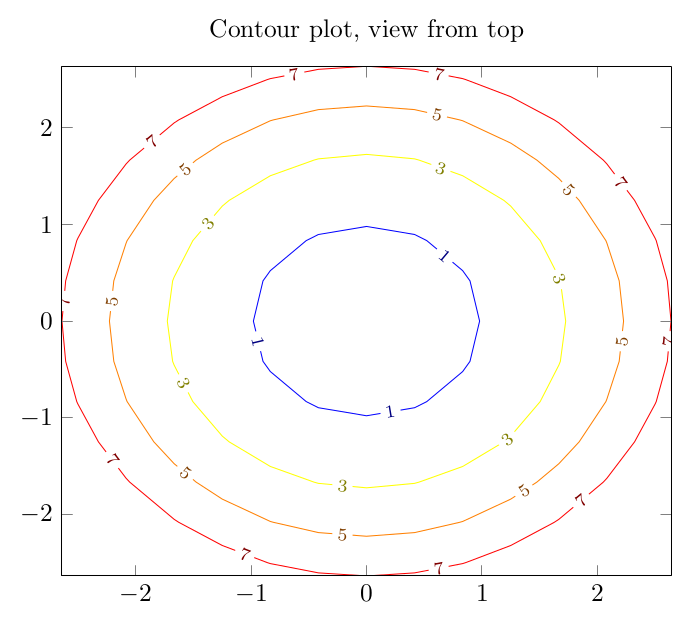
\includegraphics[scale = 0.33]{./differentialMultivariableCalculus/contour.png}
\end{figure}
\noindent
For example, the C-level surface of $f(x,y,z) = e^{-\left(x^2+y^2+z^2\right)}$ is the sphere centered at the origin with radius $\sqrt{-\ln{c}}$: $x^2 + y^2 + z^ 2 =-\ln{c}$.